\documentclass[0-thesis.tex]{subfiles}
% TODO: Entire implementation section in past tense?
\begin{document}
The previous sections proposed the update architecture of the thesis, its key components,
and security considerations such as identity and access control. This section will discuss
a prototype implementation of the architecture as well as a manifest generator. 

\subsection{Manifest Implementation}
\label{ssec:manifest-implementation}
As manifests contain certain information difficult for humans to provide such as
monotonically increasing sequence numbers and hash digests, a manifest generator was
created to help test the prototype \parencite{manifest-generator}. It is a Python script
which accepts information about vendor and class namespace, version, image file, and
associated URL in order to generate and format a manifest both in JSON and CBOR. The
outputted manifest follows the format specified in Section~\ref{ssec:manifest-format} and
features all required fields although some left blank. It is a bare-bones manifest
containing only the required information for a singular, monolithic update. There are no
dependencies or options specified.

The manifest is a JSON map featuring the required elements shown in
Figure~\ref{fig:manifest-format}. The elements are in the same order as in the figure but
the names of the fields have been substituted for integers in order to save space.
Table~\ref{tab:manifest-substitution} shows this mapping. Repeatable structures such as
preconditions are described as a nested array of maps, where each map in the array
constitutes one instance of such an element. The keys in these nested maps are also mapped
to integers as in the main manifest structure, but resetting the counter for each map. The
mapping of keys in nested structures is shown in Table~\ref{tab:nested-substitution}. The
example manifest used can be found in Appendix~\ref{app:manifest}. 

\begin{longtable}[]{@{}ll@{}}
    \caption{Mapping manifest elements to integers as keys in the JSON manifest.}
    \label{tab:manifest-substitution}\\
    \toprule
    Element Name & Mapped To\tabularnewline
    \midrule
    \endhead
    versionID & 0\tabularnewline
    sequenceNumber & 1\tabularnewline
    preConditions & 2\tabularnewline
    postConditions & 3\tabularnewline
    contentKeyMethod & 4\tabularnewline
    payloadInfo & 5\tabularnewline
    precursorImage & 6\tabularnewline
    dependencies & 7\tabularnewline
    options & 8\tabularnewline
    \bottomrule
\end{longtable}

\begin{longtable}[]{@{}ll@{}}
    \caption{Mapping elements in nested structures to integers.}
    \label{tab:nested-substitution}\\
    \toprule
    Element Name (corresponding structure) & Mapped To\tabularnewline
    \midrule
    \endhead
    type (conditions and options) & 0\tabularnewline
    value (conditions and options) & 1\tabularnewline
    \bottomrule
    URL (URL/digest pair) & 0\tabularnewline
    digest (URL/digest pair) & 1\tabularnewline
    \bottomrule
    format (payload info) & 0\tabularnewline
    size (payload info) & 1\tabularnewline
    storage (payload info) & 2\tabularnewline
    URL/digest pair (payload info) & 3\tabularnewline
    \bottomrule
\end{longtable}

In the client code, the manifest is received as a string, still formatted as JSON. In
order to parse it, structs resembling the format of the manifest were created, see
Listing~\ref{lst:manifest}. The base manifest structure contains values of version ID,
sequence number, and content key method alongside pointers to other parts of the manifest.
These parts, represented as repeated maps in the JSON string, are implemented as linked
lists in order to store an arbitrary amount of such structures. With the example manifest
shown in Appendix~\ref{app:manifest}, the base manifest structure would for instance
contain a two element long linked list of preconditions (vendor ID then class ID). Certain
manifest elements, namely precursor image, dependencies, and URL/digest pair in payload
info convey the same kind of information but are separated into different lists because of
the differences in semantics.

% TODO: Format nicely
\begin{lstlisting}[language=manifest, caption={The client manifest implementation}, label=lst:manifest]
    typedef struct manifest_s {
        uint8_t versionID;
        uint32_t sequenceNumber;
        struct condition_s *preConditions;
        struct condition_s *postConditions;
        uint8_t contentKeyMethod;
        struct payloadInfo_s *payloadInfo;
        struct URLDigest_s *precursorImage;
        struct URLDigest_s *dependencies;
        struct option_s *options;
    } manifest_t;

    typedef struct condition_s {
        int8_t type;
        char *value;
        struct condition_s *next;
    } condition_t;

    typedef struct payloadInfo_s {
        uint8_t format;
        uint32_t size;
        uint8_t storage;
        struct URLDigest_s *URLDigest;
    } payloadInfo_t;

    typedef struct URLDigest_s {
        char *URL;
        char *digest;
        struct URLDigest_s *next;
    } URLDigest_t;

    typedef struct option_s {
        int8_t type;
        char *value;
        struct option_s *next;
    } option_t;
\end{lstlisting}


\subsection{Prototype Implementation}
\label{ssec:prototype-implementation}
The prototype used in the thesis is developed in order to measure the efficiency of
transport during an update procedure as well as serving as a source of inspiration for
other implementers. It consists of a server and a client both implemented in Contiki-NG,
thus written purely in C. The prototype uses a pull model meaning the client initiates the
update procedure and the server responds with a corresponding resource. The server is
implemented in Contiki-NG as a proof-of-concept that a more capable IoT device could be
used as an update server.

% TODO: Check what I've already written about COSE in Contiki-NG (previous section)
The prototype makes use of CoAPs over DTLS with COSE encryption of payloads. Ideally COSE
would be used for signing payloads as confidentiality is already provided by DTLS, but
COSE implementations in Contiki-NG are limited and at the time of development did not
support signing. Implementing COSE signing would prove too time consuming for a project of
this scope, thus COSE encryption is used instead as a proof-of-concept of using COSE in
the update architecture. Encrypting via COSE requires more information than signing such
as nonces and Additional Authenticated Data, these have been hard-coded into the client
and server. The key has also been hard-coded. Furthermore, certificate support in
Contiki-NG is lacking and the prototype thus uses hard-coded pre-shared keys in order to
use DTLS. The last assumption made is about transferring the manifest. In the prototype
only one specific manifest is used, and thus a statically allocated buffer has been used
to make implementation easier. In a real deployment dynamic memory allocation would be
needed in order to receive and reassemble manifests of varying sizes.

% TODO: Mention registration file if I implement it
The interactions of the client and server are simplistic and the client has no other
behaviour than to initiate and complete the update procedure. As shown in
Figure~\ref{fig:client-server-interaction}, the interaction starts with a POST request
from the client to the registration endpoint of the server. The registration is sent as a
confirmable CoAP packet and is thus acknowledged by the server. Afterwards, the client
sends a GET request for a manifest. The endpoints \texttt{update/manifest} and
\texttt{update/register} are well known endpoints and all devices in the network register
and poll for manifests at these endpoints. Upon a request to \texttt{update/manifest} it
is up to the server to decide whether there is a suitable manifest or not, offloading any
decision making from the device. Since the prototype only makes use of one manifest such
logic is not implemented, but in real deployments the \texttt{update/manifest} server
resource would handle that by using the information from the devices' profile created at
the time of registration.

\begin{figure}
    \caption{The interactions of client and server during an update procedure.}
    \label{fig:client-server-interaction}
    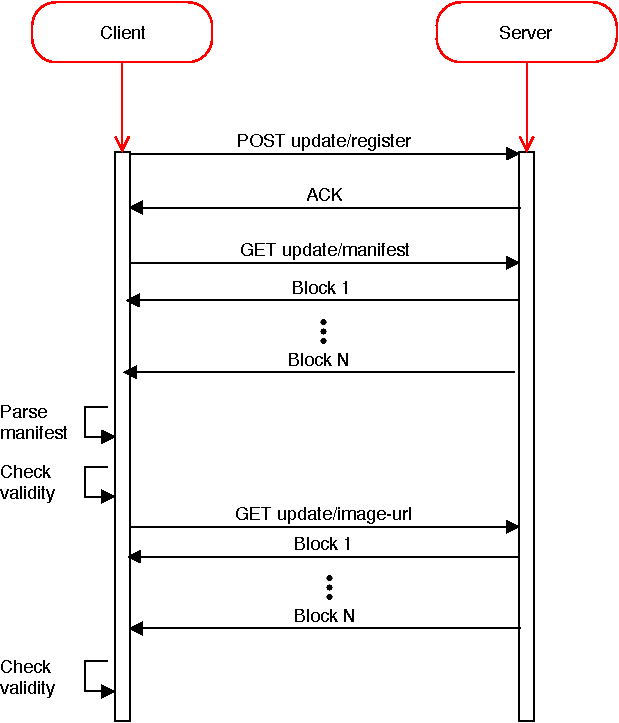
\includegraphics{images/client-server-sequence.pdf}
\end{figure}

If the server finds a suitable manifest it encodes and encrypts it using COSE and then
sends the ciphertext via CoAPs' block option. After the client has reassembled the
manifest it decrypts and decodes it, and then runs a simple parser. When the parsing is
done the client checks the preconditions to make sure it is the intended recipient by
comparing vendor and class IDs. If the client deems the manifest to be valid it requests
the update image from the URL specified in the manifest. The endpoint is now specific for
this particular class of device and version and is not known in advance, it is specified
in the manifest. After the transfer of image data has concluded the SHA-256 digest is
calculated and the procedure is finished.

The manifest and image files are encrypted in different manners for practical reasons. The
image file is relatively large and encrypting it at once requires a buffer large enough to
hold it which can prove difficult on embedded systems, whereas size requirements for the
manifest is more lax. By encrypting the image file block per block the problem of buffer
sizes is circumvented but instead introduces a larger overhead. The COSE implementation
makes use of 8 byte large tags in order to validate the ciphertext during decryption, this
means 8 of 32 bytes sent per block is overhead and not actual data. The manifest, being
encrypted in its entirety at once and then split up in blocks only introduces this
overhead once whereas the manifest transfers introduces it once per block sent. Encrypting
the image this way also requires decrypting each block instead of decrypting just once as
with the manifest. With the limited buffer sizes available however, encrypting and
decrypting the entire image file at once is not feasible using the hardware of the thesis.


\end{document}